\documentclass{article}
\usepackage[utf8]{inputenc}
\usepackage{hyperref}

\title{Übung 4}
\author{Laurenz Weixlbaumer, 11804751}
\date{November 2018}

\renewcommand\thesubsection{(\alph{subsection})}

\usepackage{enumitem}
\usepackage{mathtools}

\begin{document}

\maketitle

\stepcounter{section}
\section{Addition und Subtraktion}

\begin{enumerate}[label=(\alph*)]

\item Subtraktion von Binärzahlen im Zweierkomplement.

\begin{tabular}{ c c c c c }
      & 1 & 0 & 1 & 0 \\
    - & 0 & 1 & 0 & 1 \\
    \hline
      & 0 & 1 & 0 & 1
\end{tabular}

\begin{tabular}{ c c c c c c }
      & 1 & 1 & 0 & 0 & 0 \\
    - & 0 & 1 & 1 & 1 & 0 \\
    \hline
      & 0 & 1 & 0 & 1 & 0
\end{tabular}

\item Wahrheitstabelle eines 1-Bit Vollsubtrahierers.

\begin{tabular}{ c c c | c c }
    a & b & $B_i$ & D & $B_o$ \\
    \hline
    0 & 0 & 0 & 0 & 0  \\
    0 & 0 & 1 & 1 & 1  \\
    0 & 1 & 0 & 1 & 1  \\
    0 & 1 & 1 & 0 & 1  \\
    1 & 0 & 0 & 1 & 0  \\
    1 & 0 & 1 & 0 & 0  \\
    1 & 1 & 0 & 0 & 0  \\
    1 & 1 & 1 & 1 & 1
\end{tabular}

\clearpage

\item 4-Bit Additions-Subtraktionswerk

\begin{figure}[h]
\begin{center}
    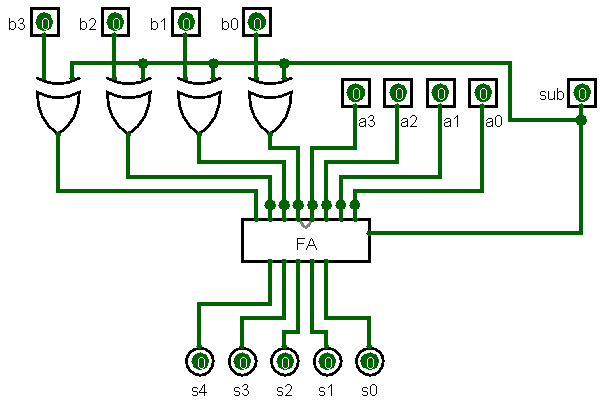
\includegraphics[width=12cm]{addsub_circuit.png}
    4-Bit Additions-Subtraktionswerk Schaltbild
\end{center}
\end{figure}

Auf der nächsten Seite wird das Werk verwendet um $1101_2$ von $1001_2$ zu subtrahieren, die Pegel an den Ein- und Ausgängen, Addierern und Gattern sind farblich hervorgehoben.

\begin{figure}[t]
\begin{center}
    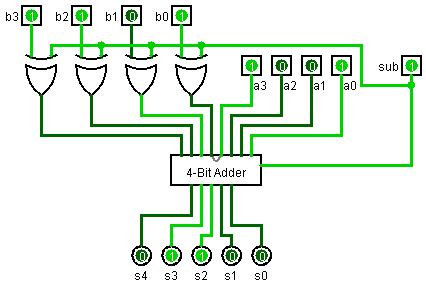
\includegraphics[width=12cm]{addsub_main_circuit_marked.png}
    Hauptschaltkreis
\end{center}
\end{figure}

\begin{figure}[t]
\begin{center}
    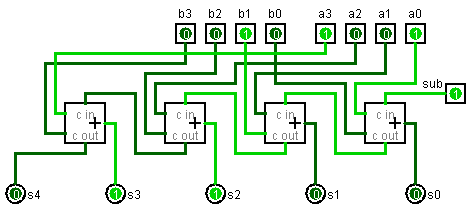
\includegraphics[width=12cm]{addsub_blck_circuit_marked.png}
    4-Bit Addierer
\end{center}
\end{figure}

\end{enumerate}

\end{document}
